\subsection{Testing}
\subsubsection{Analisi Statica - CodMR}

L'analisi statica del codice è stata gestita tramite il tool CodeMR.

\begin{figure}[H]
    \centering
    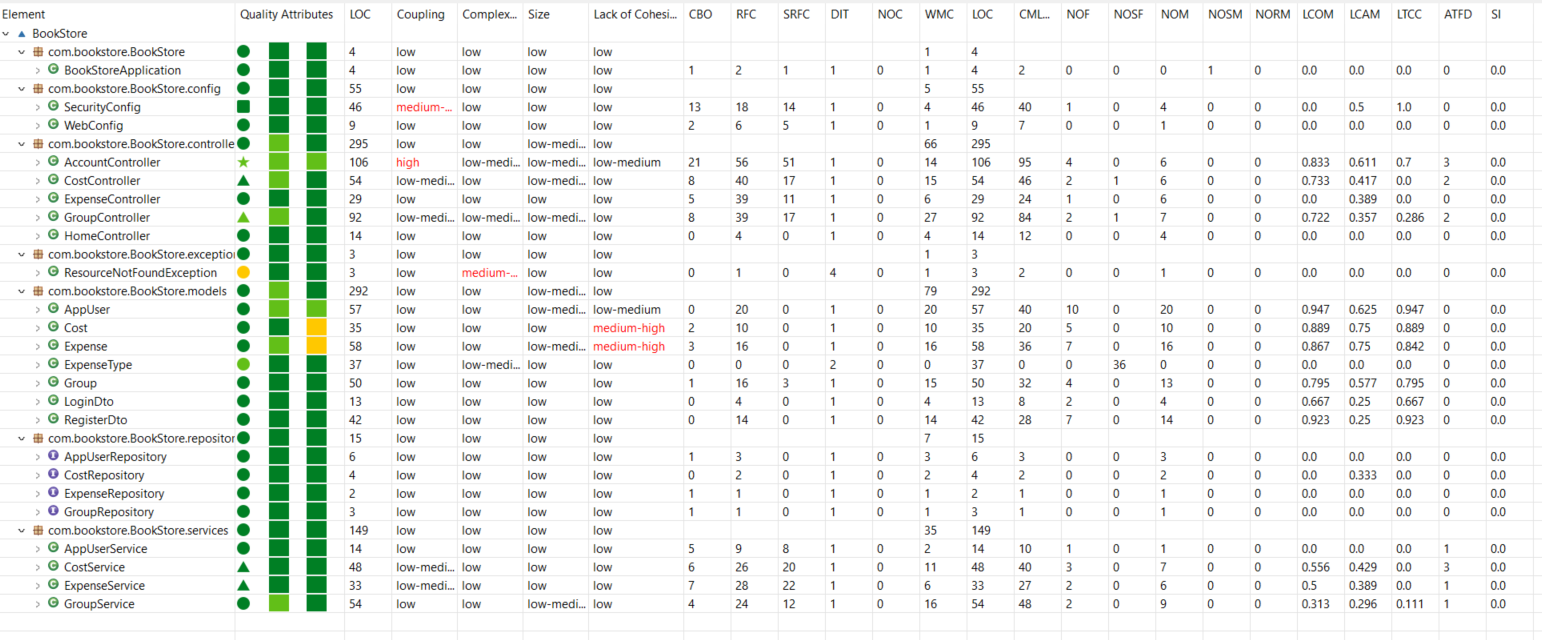
\includegraphics[width=0.9\textwidth]{images/CodeMR_graph1.png}
    \caption{Metriche del progetto}
    \label{fig:CodeMR_1}
\end{figure}

Dall'analisi dell'immagine si può notare che i livelli di coupling e complexity sono tendelzialmente bassi.
Per quanto riguarda il coupling, solo le classi SecurityConfig e AccountController presentano dei valori medio-alti. 
Invece, per la complessità l'unica classe con un valore elevato è la ResourceNotFoundException.

\begin{figure}[H]
    \centering
    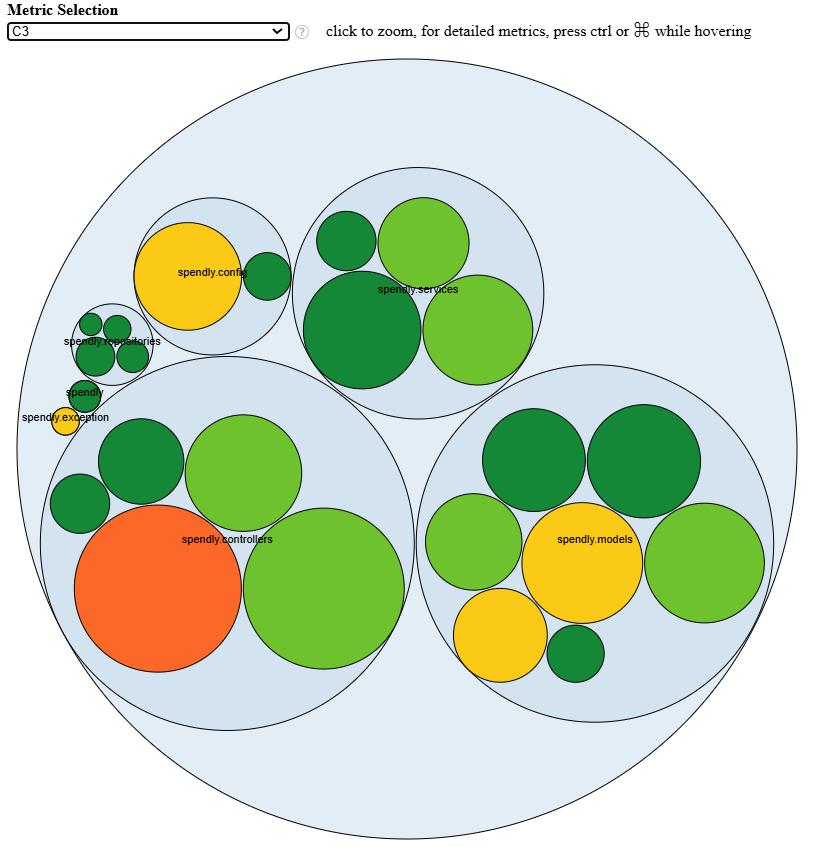
\includegraphics[width=0.6\textwidth]{images/CodeMR_graph2.png}
    \caption{Struttura dei package}
    \label{fig:CodeMR_2}
\end{figure}


\subsubsection{Analisi Dinamica - JUnit}

L'analisi dinamica del codice è stata condotta utilizzando JUnit per l'esecuzione di test automatizzati sui metodi delle principali classi, e Postman per verificare il corretto funzionamento delle API implementate nei controller.
In particolare, con JUnit sono stati sviluppati test specifici per validare i metodi delle classi relative alla gestione dei gruppi, quali Group, GroupService e GroupController.

\begin{figure}[H]
    \centering
    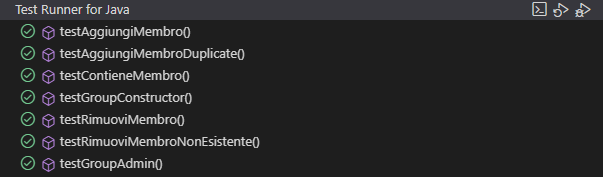
\includegraphics[width=0.9\textwidth]{images/TestGroup.png}
    \caption{Test per la classe Group}
    \label{fig:Group_test}
\end{figure}

\begin{figure}[H]
    \centering
    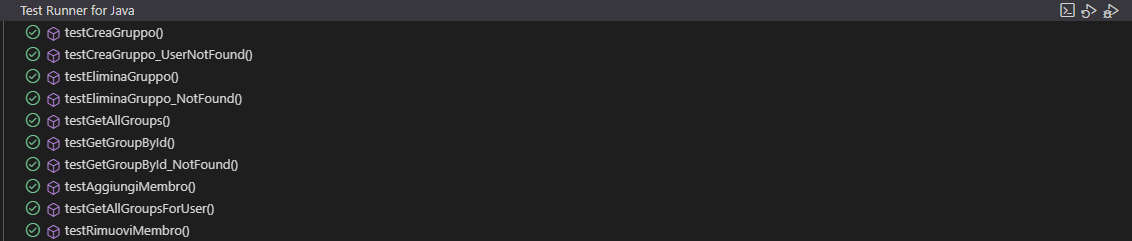
\includegraphics[width=0.9\textwidth]{images/TestGroupService.png}
    \caption{Test per la classe GroupService}
    \label{fig:GroupService_test}
\end{figure}

\begin{figure}[H]
    \centering
    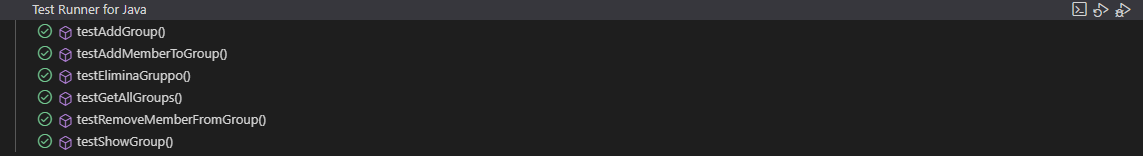
\includegraphics[width=0.9\textwidth]{images/TestGroupController.png}
    \caption{Test per la classe GroupController}
    \label{fig:GroupController_test}
\end{figure}


\subsubsection{API Esposte}

Questa sezione documenta le API principali del sistema \textbf{Spendly}, includendo autenticazione, gestione dei gruppi e visualizzazione. Ogni test verrà mostrato con un' \texttt{immagine dei risultati}.

\paragraph{Registrazione Utente}
\begin{itemize}
    \item \textbf{Endpoint:} \texttt{POST /account/register}
    \item \textbf{Descrizione:} Consente a un nuovo utente di registrarsi al sistema.
    \item \textbf{Parametri:}
    \begin{itemize}
        \item \texttt{nome} (string) - Nome utente.
        \item \texttt{cognome} (string) - Nome utente.
        \item \texttt{username} (string) - Username utente(non accetta duplicati).
        \item \texttt{email} (string) - Email dell'utente(non accetta duplicati).
        \item \texttt{telefono} (string) - Telefono utente.
        \item \texttt{indirizzo} (string) - Indirizzo utente.
        \item \texttt{password} (string) - Password scelta dall'utente.
    \end{itemize}
    \item \textbf{Risultato:}
\end{itemize}
\begin{figure}[H]
    \centering
    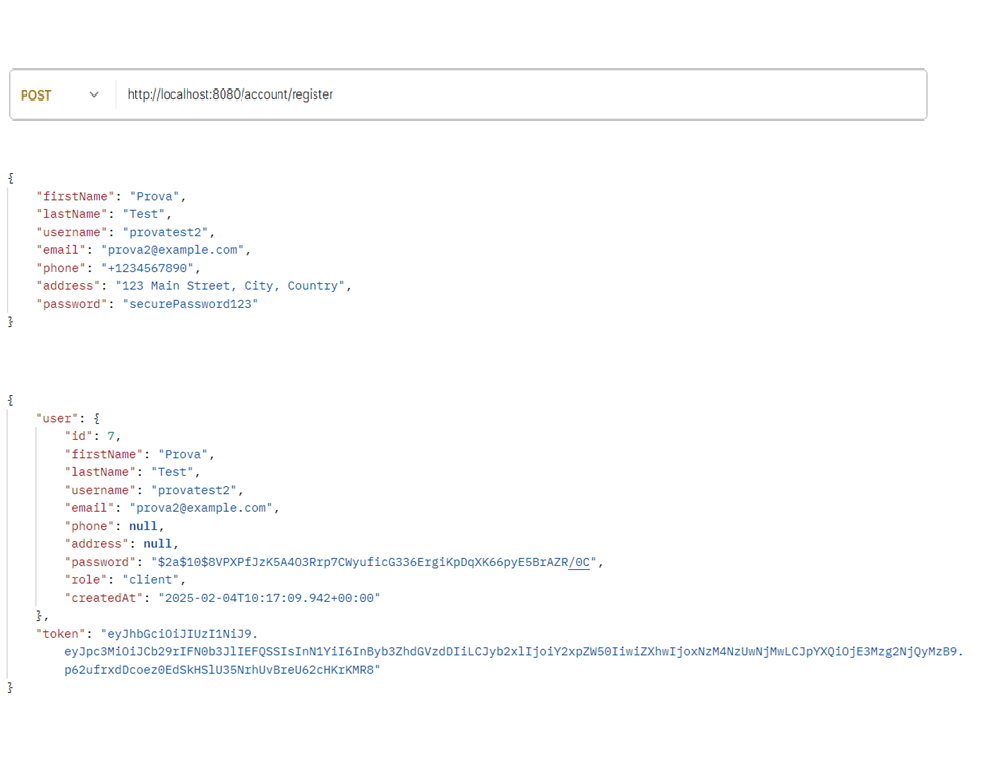
\includegraphics[width=0.9\textwidth]{images/registerapi.png}
    \caption{Risultato API Registrazione}
    \label{fig:api_register}
\end{figure}

\paragraph{Login Utente}
\begin{itemize}
    \item \textbf{Endpoint:} \texttt{POST /account/login}
    \item \textbf{Descrizione:} Permette a un utente registrato di accedere al sistema.
    \item \textbf{Parametri:}
    \begin{itemize}
        \item \texttt{username} (string) - Username dell'utente.
        \item \texttt{password} (string) - Password dell'utente.
    \end{itemize}
    \item \textbf{Risultato:}  
\end{itemize}
\begin{figure}[H]
    \centering
    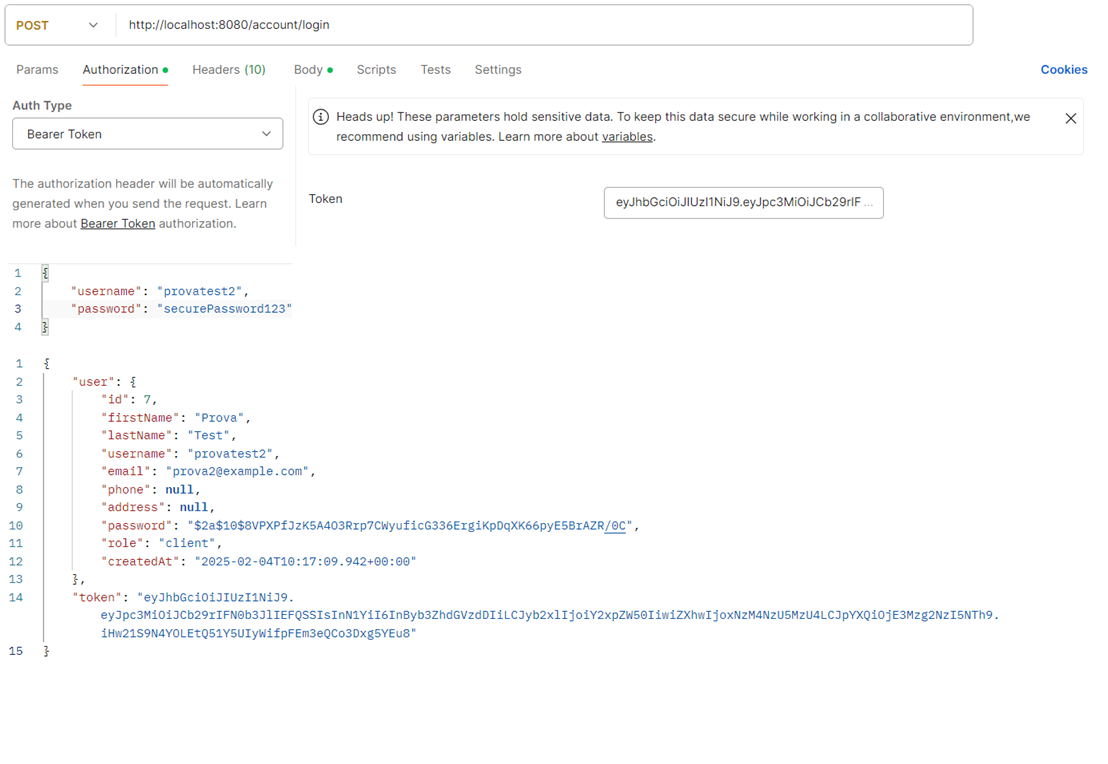
\includegraphics[width=0.9\textwidth]{images/loginapi.png}
    \caption{Risultato API Login}
    \label{fig:api_login}
\end{figure}

\paragraph{Creazione di un Gruppo}
\begin{itemize}
    \item \textbf{Endpoint:} \texttt{POST /api/groups}
    \item \textbf{Descrizione:} Permette la creazione di un nuovo gruppo da parte dell'utente.
    \item \textbf{Parametri:}
    \begin{itemize}
        \item \texttt{name} (string) - Nome del gruppo.
        \item \texttt{username} (string) - Username dell'utente che crea il gruppo.
    \end{itemize}
    \item \textbf{Risultato:}
\end{itemize}
\begin{figure}[H]
    \centering
    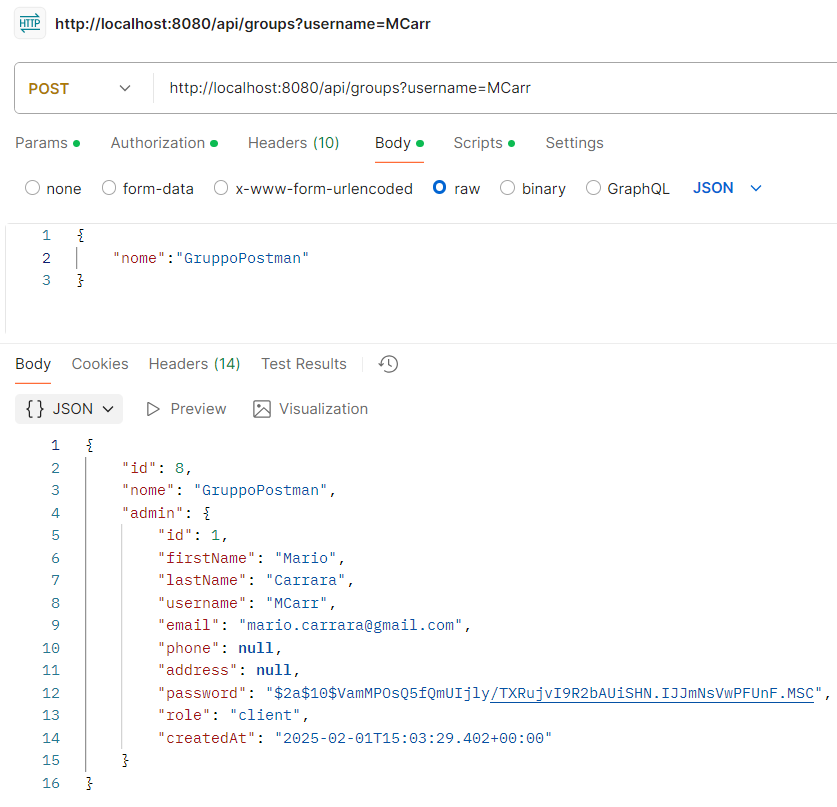
\includegraphics[width=0.8\textwidth]{images/CreateGroupAPI.png}
    \caption{Risultato API Creazione Gruppo}
    \label{fig:api_create_group}
\end{figure}

\paragraph{Inserimento di un utente in un gruppo}
\begin{itemize}
    \item \textbf{Endpoint:} \texttt{POST /api/groups/{group\_id}/members}
    \item \textbf{Descrizione:} Permette all'amministratore di inserire un utente in un gruppo.
    \item \textbf{Parametri:}
    \begin{itemize}
        \item \texttt{adminUsername} (string) - Username dell'admin del gruppo.
        \item \texttt{memberUsername} (string) - Username dell'utente da inserire.
    \end{itemize}
    \item \textbf{Risultato:}
\end{itemize}
\begin{figure}[H]
    \centering
    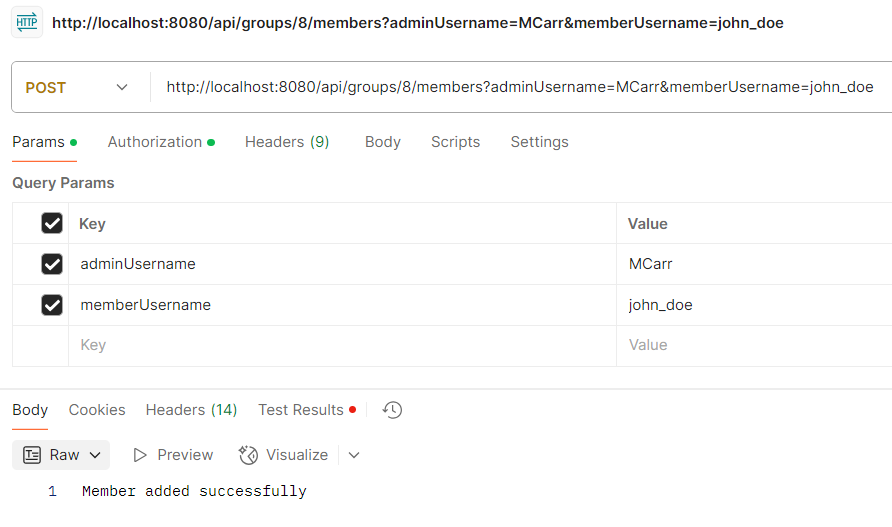
\includegraphics[width=0.8\textwidth]{images/AddMemberAPI.png}
    \caption{Risultato API Inserimento utente}
    \label{fig:api_add_member}
\end{figure}

\paragraph{Visualizzazione dei Gruppi}
\begin{itemize}
    \item \textbf{Endpoint:} \texttt{GET /api/groups}
    \item \textbf{Descrizione:} Restituisce la lista di tutti i gruppi a cui l'utente appartiene.
    \item \textbf{Parametri:}
    \begin{itemize}
        \item \texttt{username} (string) - Username dell'utente.
    \end{itemize}
    \item \textbf{Risultato:}
\end{itemize}
\begin{figure}[H]
    \centering
    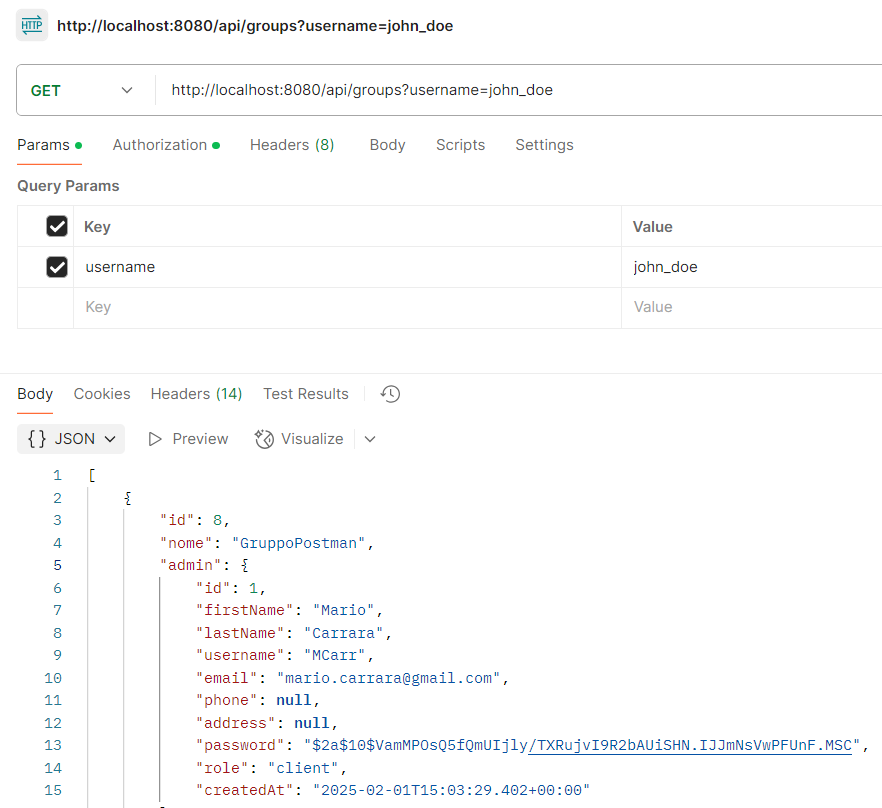
\includegraphics[width=0.8\textwidth]{images/GetAPI.png}
    \caption{Risultato API Visualizzazione Gruppi}
    \label{fig:api_view_groups}
\end{figure}

